\section{Algorithm/Concept}
\label{sec:algorithm}
\graphicspath{{utils/}}
As this Bachelor Thesis tackles two problems, the algorithms can be divided into two categories as well.
The first category consists of racing line recording concepts and the second one of ways to compare these recordings.

\subsection{Recording}
\subsubsection{Visual Odometry}
Visual Odometry (VO) is a concept that most camera-based robots use for navigation. It uses two consecutive camera frames to calculate the rotation and translation of the camera between them. The advantage over traditional tracking systems like GPS is, that it isn't dependent on any external sources, like satellites or radio towers, to determine the position of the object.
Also it is capable of much higher polling rates than most GPS receivers, which normally poll at 1 Hz, so they get 1 positional update per second. The potential speed of Visual Odometry is linked to the frame rate of the camera. That way, a camera that records at 30 frames per second enables Visual Odometry to estimate a position 30 times a second. 
The crude algorithm behind VO determines and stores recognizable features in one frame, using a feature detection algorithm.
At first we need two consecutive, rectified camera images. It is important that the images are rectified, because otherwise the edges of the image would be curved and produce wrong results.
Our solution uses the Harris corner detection method for determining features. Finding corners in an image is a very important prerequisite for the final position determination, because it allows us to calculate direction vector to another point. This other point being the same feature in the following camera frame, where the Harris detector is used, as well.
Having two sets of corners from either image we can track each feature from one frame to another. 
\begin{itemize}
    \item Lucas-Kanade?
    \item Jacobian?
\end{itemize}
Now that we have an end point to every (possible) starting point, we can construct a set of directional vectors.
Removing outliers (i.e. vectors that are much longer or go in a vastly different direction than most vectors) an approximation translation and rotation the camera conducted during the two frames can be calculated.
Outlier removal is important, because otherwise the movement of other cars on the track would cause the algorithm to think the camera was moving in a different direction than it actually was.
If the taken path includes loops it is possible to optimize the result by using loop detection. If any features are re-detected at a later point in time and the current position is close to the position the features were re-detected, the path can be stretched in a way that it connects to the earlier path.
This can reduce errors that accumulated due to small estimation errors in the previous steps.

%%%%%%%%%%%%%%%%%%%%%%%%%%%%%%%%%%%%%%%%%%%%%%%%%%%%%%%%%%%%%%%%%%%%%%%%%
%TODO:
%\begin{itemize}
%  \item track features from one image to another (Lucas-Kanade-Method)
%  \item approximate direction vector based on emerging vectors (RANSAC?)
%  \item optimize result (Loop-Detection, Algorithm)
%\end{itemize}

\subsubsection{Lane Detection}
Lane Detection uses markings on a road to determine its lateral boundaries in relation to the recording camera. It is often used in autonomous driving and driving assistance systems, because the position of the car in between lane markings gives a lot of information about the direction the car is traveling. 
In our case, not only can we determine a traveling direction, but also the position on the lane.
By tracking the distance to the left and right lane, a deviation to the middle of the lane can be calculated. 
If the driven track is know or the camera is capable of determining a scale (e.g. by using a stereo camera), the deviation can even be expressed as a metric length, which is helpful for extracting additional information, like speed and acceleration, later on.


%TODO: Algorithms
\begin{itemize}
  \item possibility to improve recording results on known track
  \item possibility to determine accurate horizontal position on track
\end{itemize}

\subsubsection{Recording OBD2 Data}
\textit{Definition} OBD II (On-board diagnostics 2) is an interface which all cars build after 1996 in the USA or after 2003 in the EU, respectively, have to have built-in. It implements the SAE J1962 standard which provides standardized PIDs that return specific car-based sensor data, like the current speed, current motor revolution (rpm), throttle position and more.
A data request is possible about 10 times per second. This gives us a good basis for further detailed comparisons combined with the racing line recording.

\subsection{Comparing}
\subsubsection{Visual Comparison of Racing Line with help of sensor data}
A fairly simple, but effective way to find out where time is lost on the track is the visual comparison of racing lines from different drivers. The idea is to overlay the previously recorded lines over the race track. To actually determine at which point a driver was faster than the other one, we need an obvious optical representation of the speed at any given point on the track and the possibility to receive further information on demand.
In our system, the speed is represented by coloring in the racing line on a gradient scale reaching from green (standing still) to red (>250 km/h).
%TODO: Algorithm here
Besides speed data, different values, like acceleration, braking behavior or lap time, can be displayed in a similar fashion. That way the fastest line for a given corner can be determined and the slower driver can find out, why their line was inferior.

\begin{itemize}
  \item highlight relevant locations, like corners, showing detailed information about throttle and brake behavior and curvature through the corner
  \item fastest way through corner is trade-off between distance traveled and curvature, with low curvature allowing the driver to carry more speed to exit of the corner
\end{itemize}

\subsubsection{Mathematical Calculation of ideal line given a certain track}
Besides comparing two driver-generated racing lines, it is also possible to calculate a fast, almost ideal racing line.

\textit{Bézier Curves}
Bézier curves are a way to depict an entire race track, i.e. a curved path, with a set of control points, \{P\textsubscript{0}, P\textsubscript{1}, ..., P\textsubscript{n}\}. In this definition, n is the order of the curve. P\textsubscript{0} and P\textsubscript{n} stand for the beginning and the end point of the curve, respectively, while the intermediate points define the curvature of the curve and don't usually lie on it.

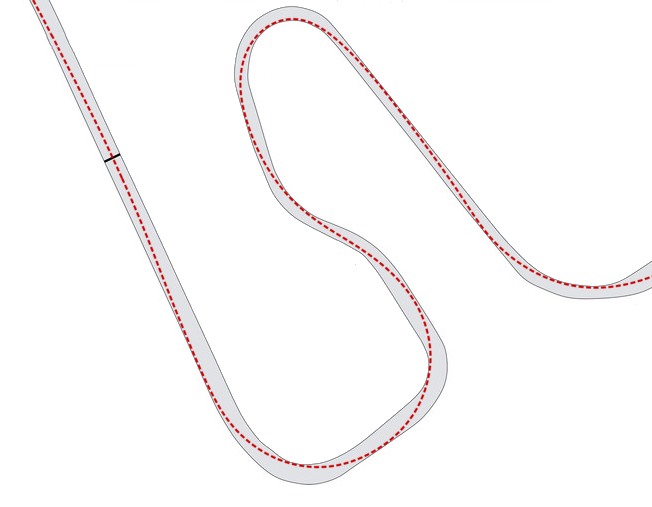
\includegraphics[width=\textwidth]{bezier_track}

\begin{itemize}
  \item calculating smooth curves around an edged representation of the track using Bézier curves
  \item naively not an optimized track, but fair approximation
  \item simulating a chain of spring-loaded masses -> ideal line calculated by iterating multiple times and taking the line that uses the least force to keep masses in bounds of track (//this seems quite complex, not really sure how this works yet)
\end{itemize}

\subsubsection{Mathematical Comparison of two paths}
\begin{itemize}
  \item convert pair of consecutive points into list of vectors; each vector is distance between points and angle to x-axis
  \begin{itemize}
    \item double dx = endPoint.X - startPoint.X;
    \item double dy = endPoint.Y - startPoint.Y;
    \item double magnitude = Math.Sqrt((dx * dx) + (dy * dy));
    \item double direction = Math.Atan2(dy, dx) * (180 / Math.PI);
  \end{itemize}
  \item combine vectors that have the same direction, by generating a new vector with the direction of the old ones and the sum of their lengths. This indicates a straight, which is not that interesting for comparison
  \item Now we can compare the angle for each section of a corner
\end{itemize}
\clearpage
